\documentclass[../main.tex]{subfiles}
\begin{document}
\paragraph{Bifurcation set}\label{par:bif_set}

\begin{figure}[H]
    \centering 
    \begin{subfigure}[b]{0.495\textwidth}
        \centering 
        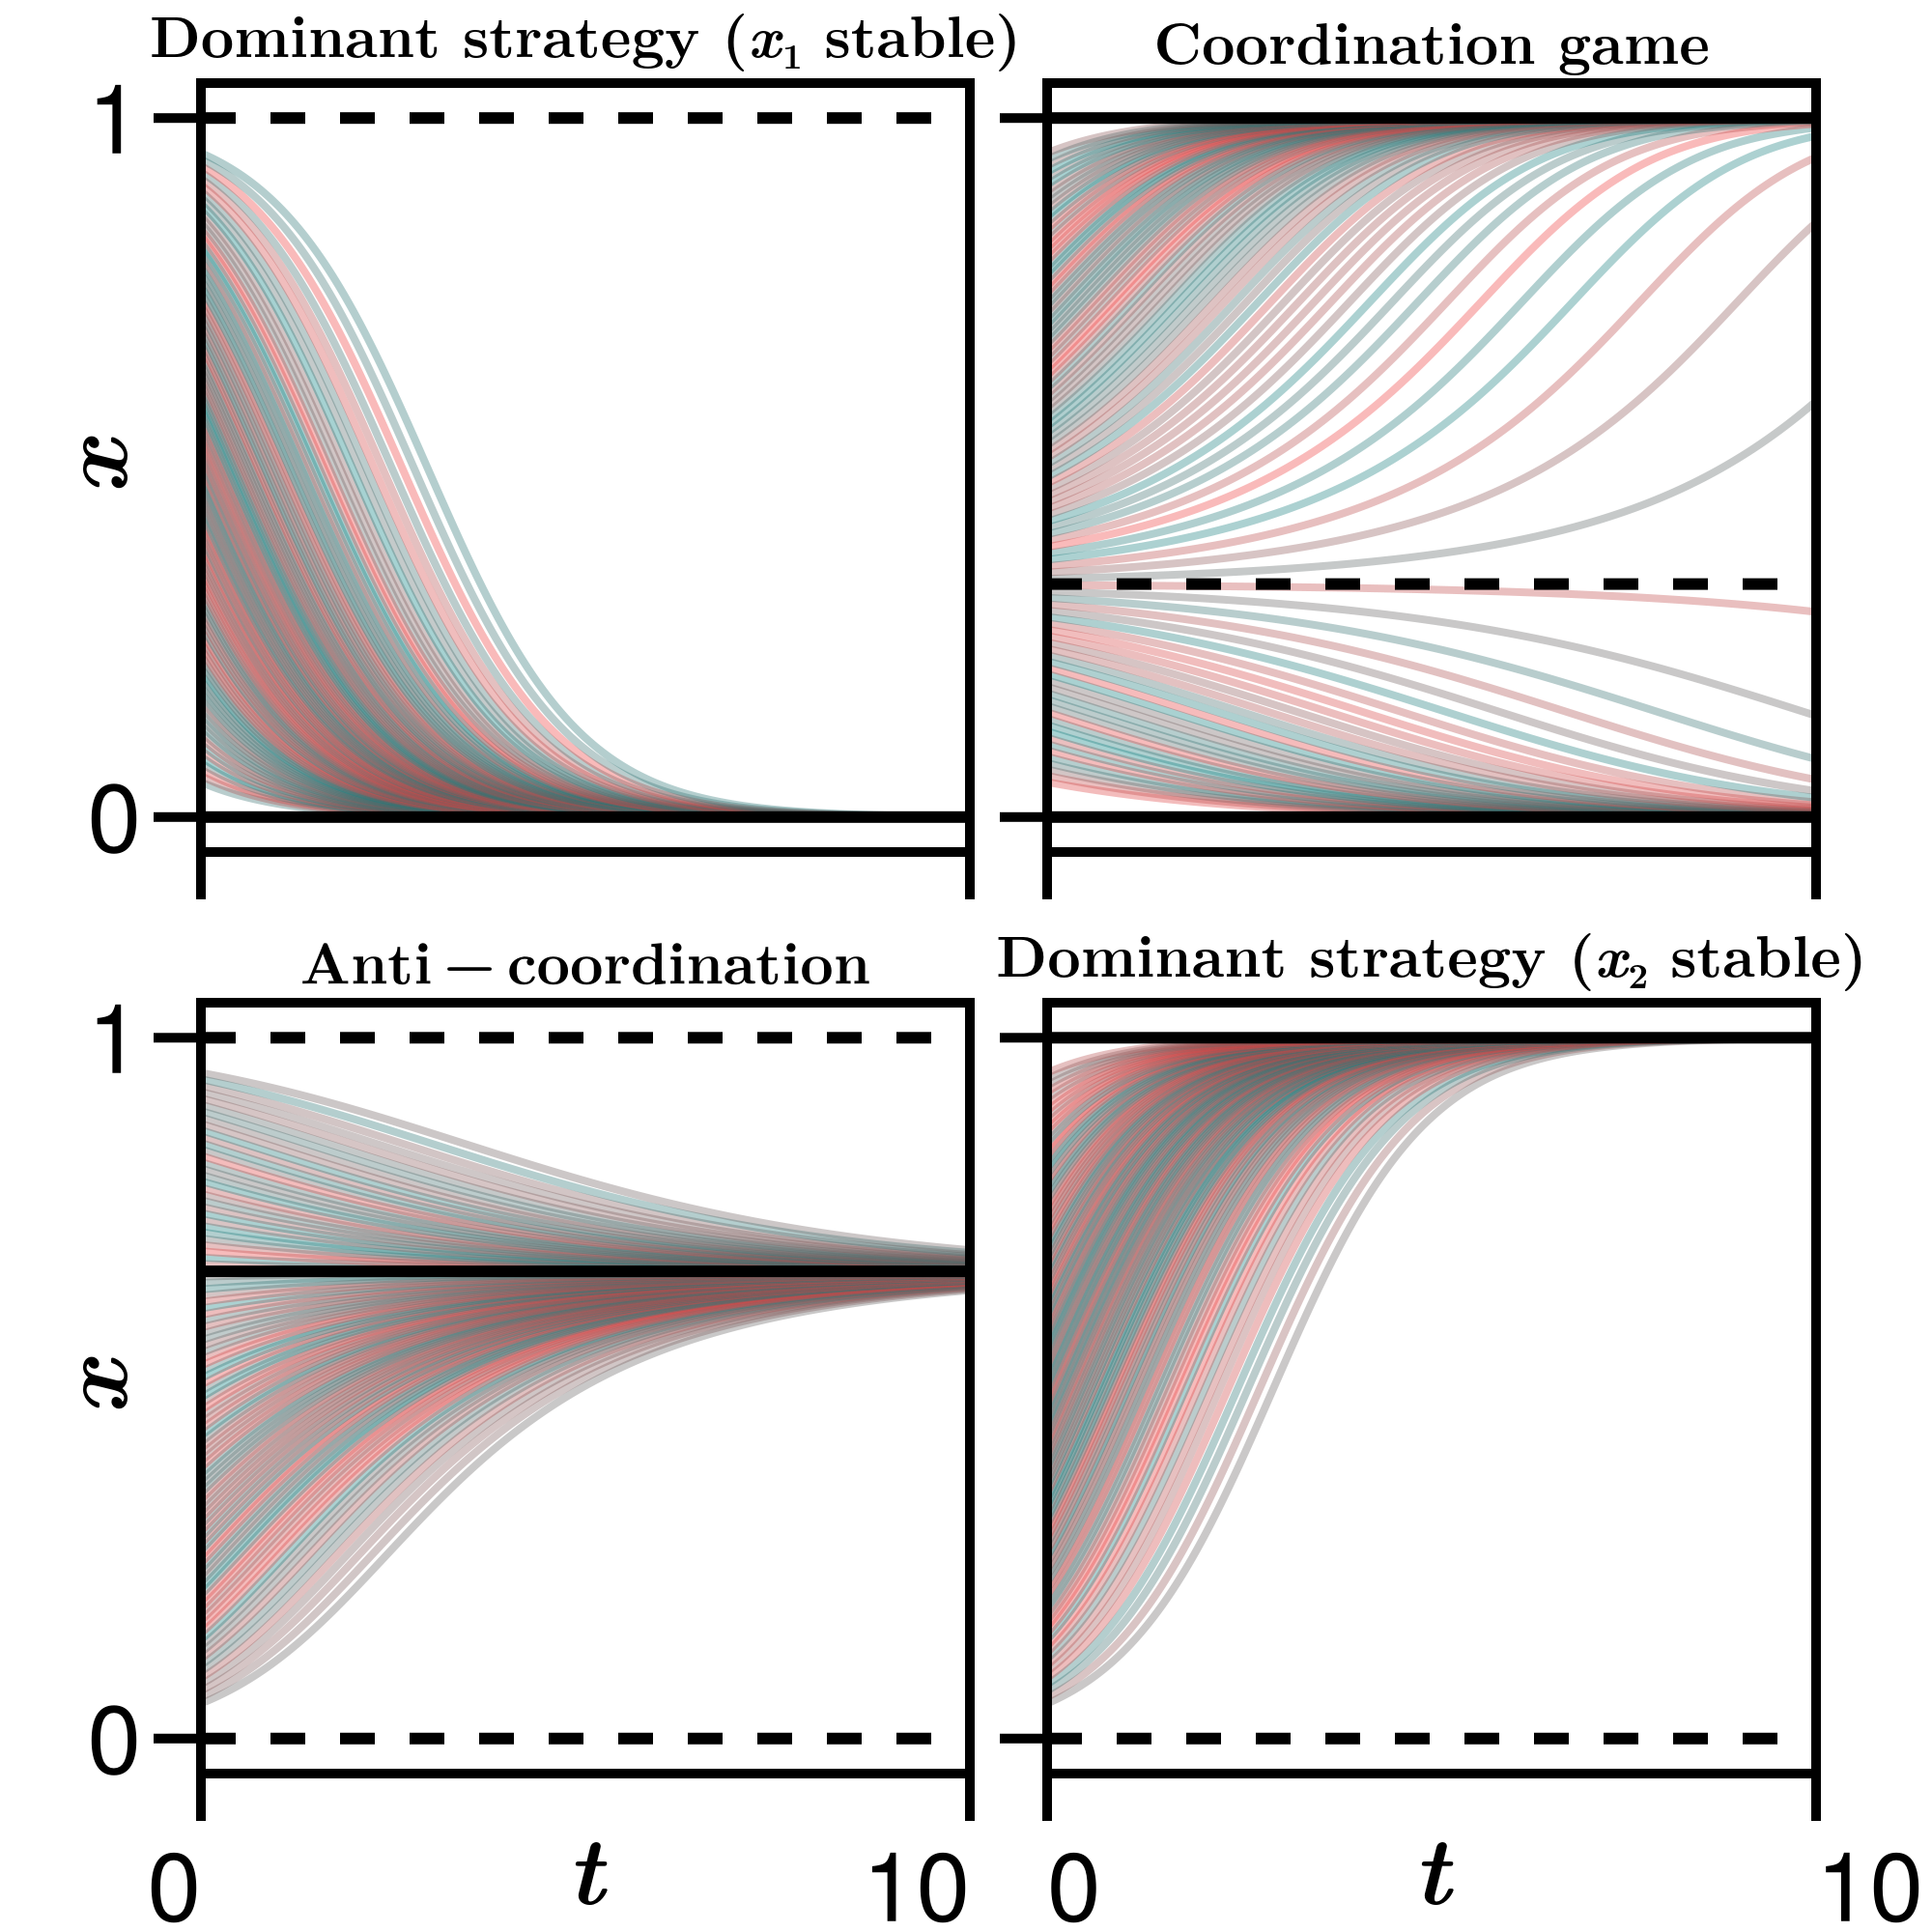
\includegraphics[keepaspectratio, width = \linewidth]{../figures/fig:autonomous_solutions.png}
        \caption{}
        \label{fig:autonomous_solutions}
    \end{subfigure}
    \hfill
    \begin{subfigure}[b]{0.495\textwidth}
        \centering 
        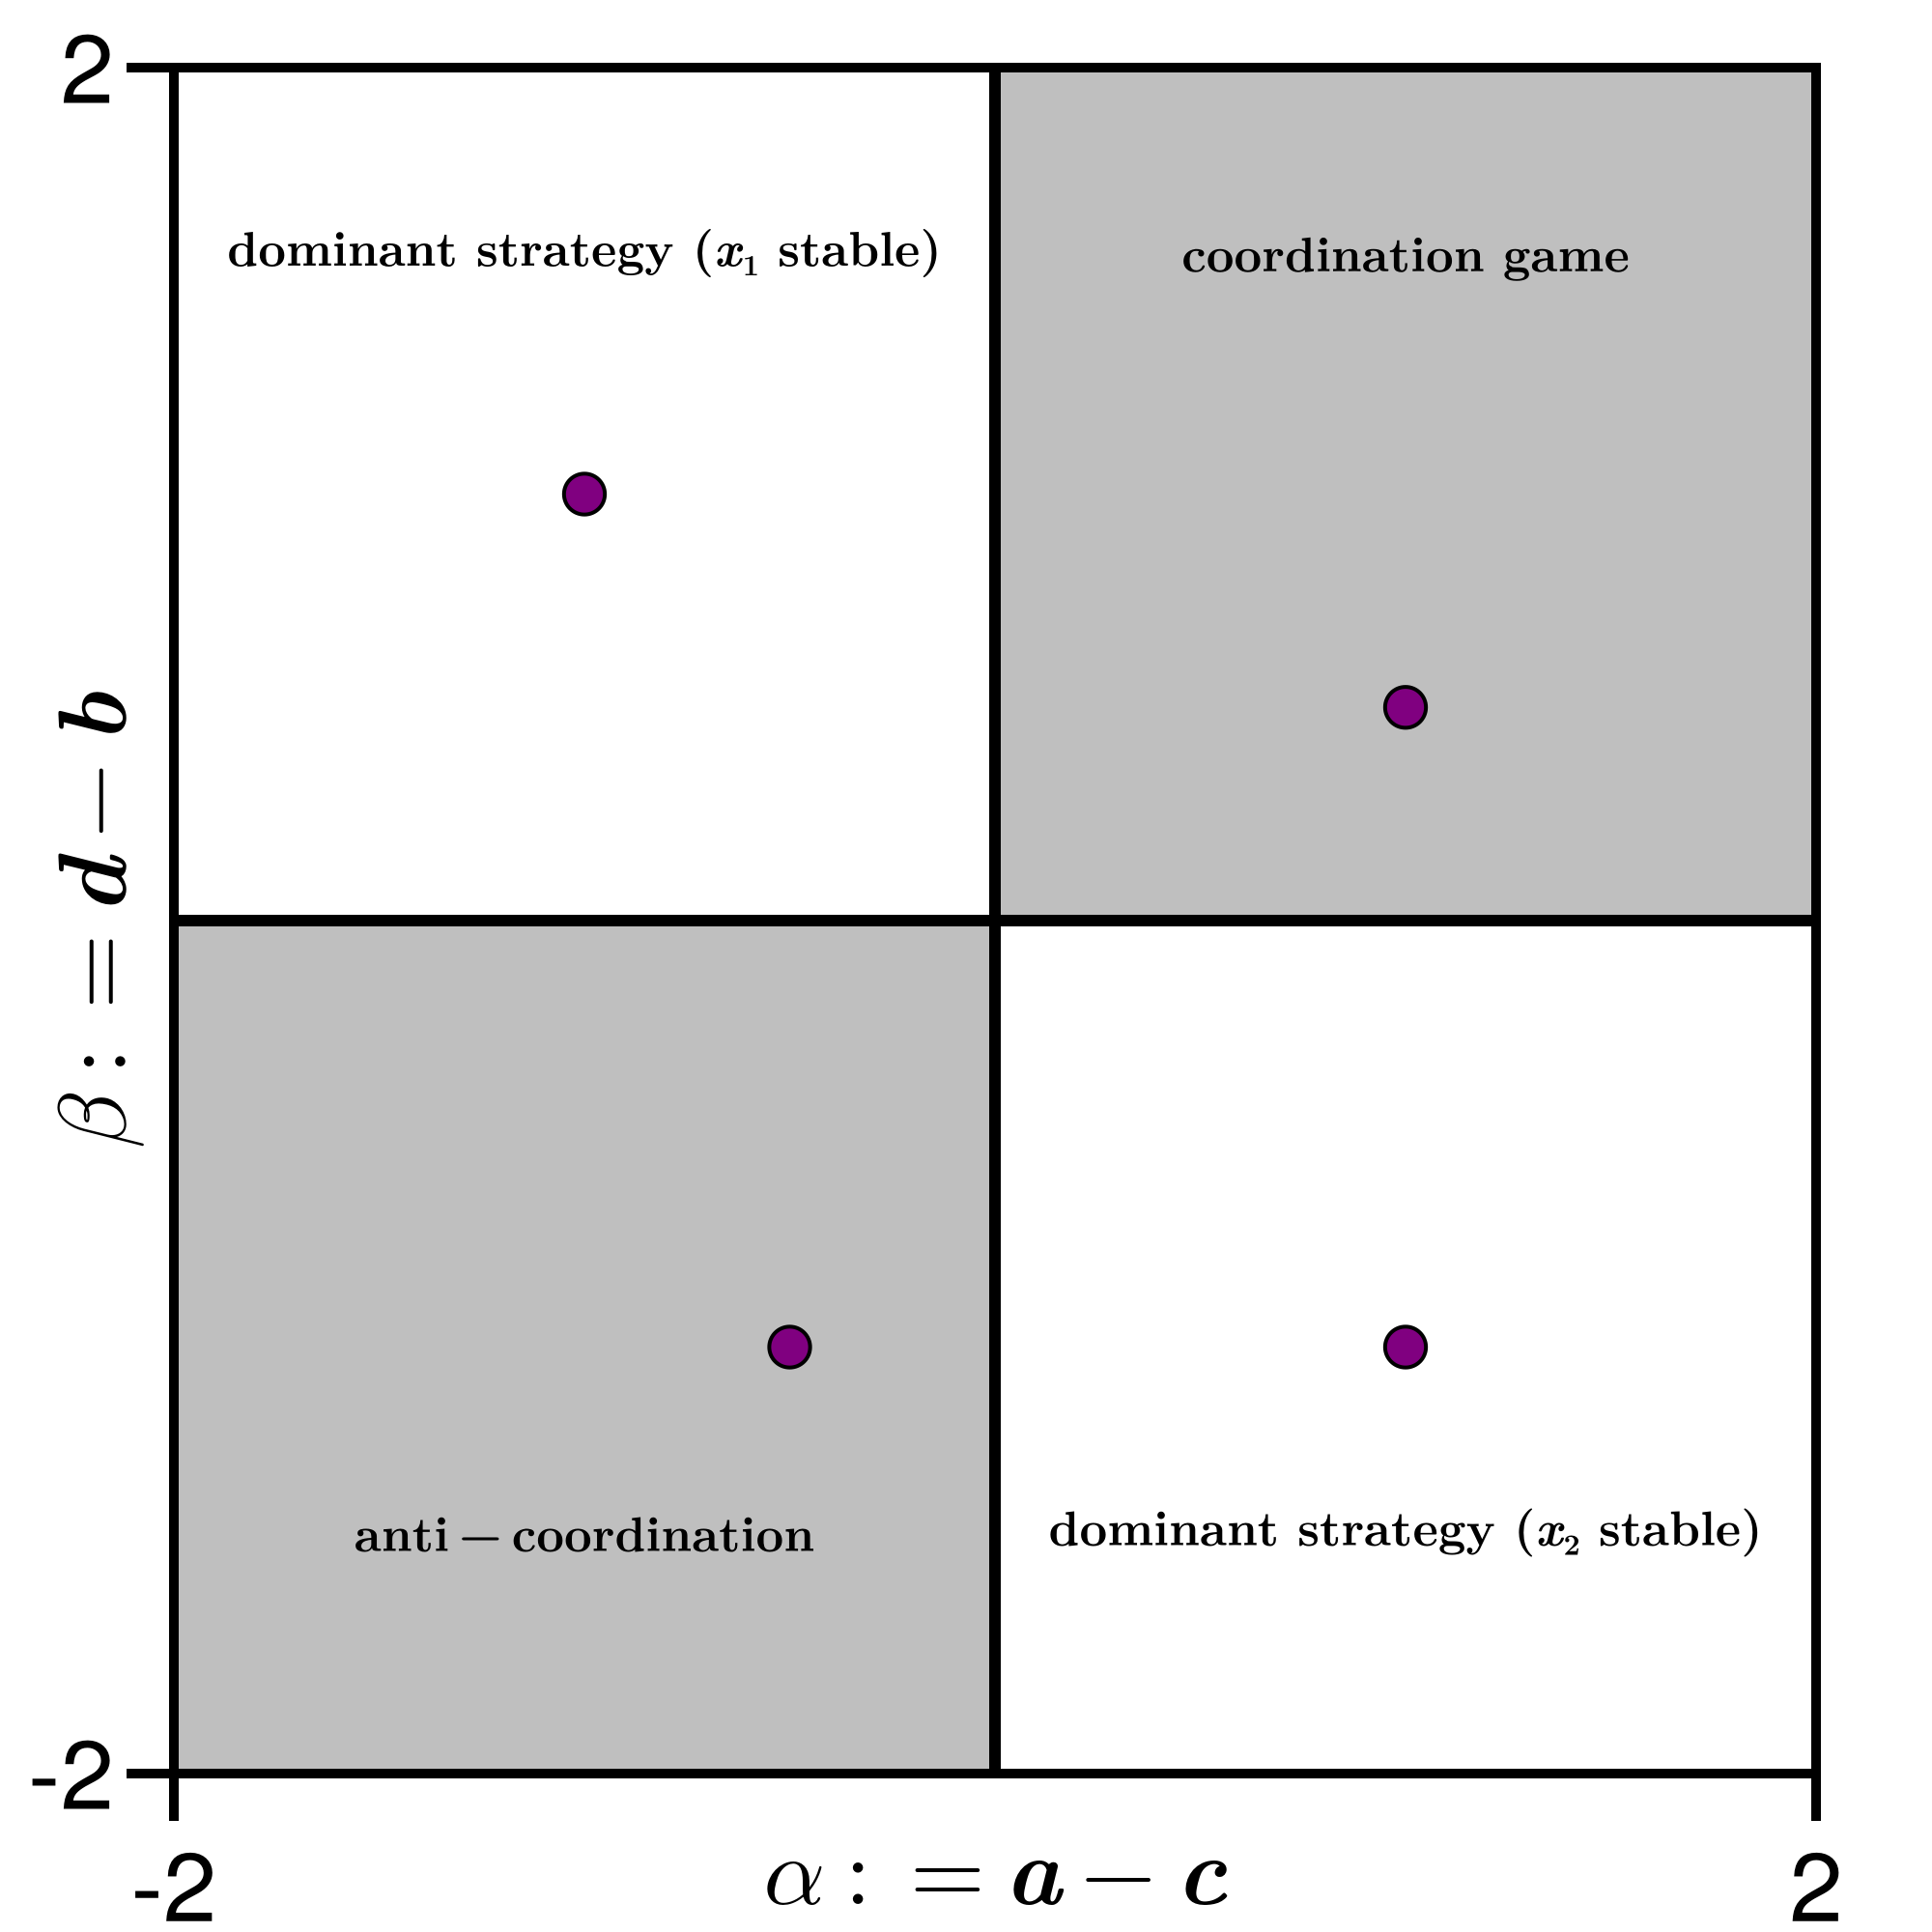
\includegraphics[keepaspectratio, width = \linewidth]{../figures/fig:autonomous_bifset.png}
        \caption{}
        \label{fig:autonomous_bifset}
    \end{subfigure}

    \caption{Properties of the autonomous system \eqref{eq:replicator_implicit} in qualitatively different regions of the admissable set $\Gamma$ as per Lemma \ref{lemma:stability}.
            (a) Asymptotic stability in $\Omega$ of different initial conditions for qualitatively different values of the parameter vector $\gamma:=(\alpha,\beta)\in\Gamma$. 
            Solid black lines indicate globally stable equilibria; dashed black lines indicate globally unstable equilibria. 
            (b) Bifurcation set in $\mathbb{R}^{2}$ with separatrices (solid black lines) indicating the transcritical bifurcations outlined in Theorem \ref{thm:bifurcations}.
            Purple dots in each region indicate the position in the admissable set ($\Gamma_{*}\subset\Gamma$ is shaded in gray) for which the solutions on the left are plotted.
    }
    \label{fig:autonomous}
\end{figure}

% 
%\subfile{subpar:}

\end{document}
